\documentclass[parskip=full]{scrartcl}
\usepackage[margin=2cm,paperheight=40cm]{geometry}
\usepackage{tikz}

\newcommand\DrawControl[3]{
  node[#2,circle,fill=#2,inner sep=2pt,label={above:$#1$},label={[black]below:{\footnotesize#3}}] at #1 {}
}

\pagestyle{empty}

\begin{document}
\centering

One control point:\\
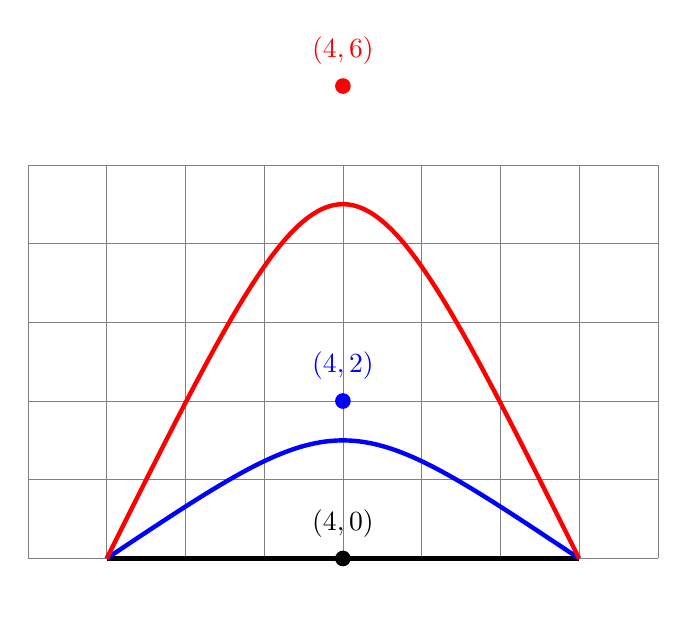
\begin{tikzpicture}[baseline]
\draw[help lines] (0,0) grid (8,5);
\draw[ultra thick] 
  (1,0) 
    .. controls (4,0) .. 
  (7,0) \DrawControl{(4,0)}{black}{};  
\draw[ultra thick,blue] 
  (1,0) 
    .. controls (4,2) .. 
  (7,0) \DrawControl{(4,2)}{blue}{};  
\draw[ultra thick,red] 
  (1,0) 
    .. controls (4,6) .. 
  (7,0) \DrawControl{(4,6)}{red}{};  
\end{tikzpicture}\hfill
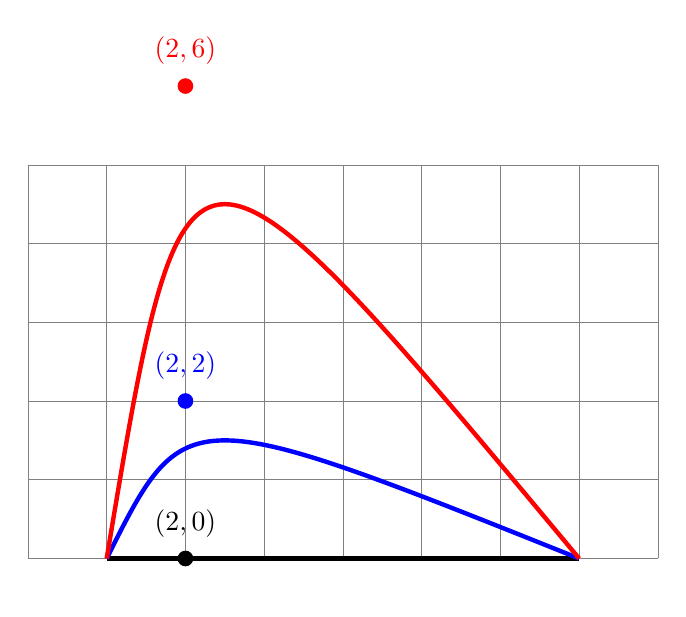
\begin{tikzpicture}[baseline]
\draw[help lines] (0,0) grid (8,5);
\draw[ultra thick] 
  (1,0) 
    .. controls (2,0) .. 
  (7,0) \DrawControl{(2,0)}{black}{};  
\draw[ultra thick,blue] 
  (1,0) 
    .. controls (2,2) .. 
  (7,0) \DrawControl{(2,2)}{blue}{};  
\draw[ultra thick,red] 
  (1,0) 
    .. controls (2,6) .. 
  (7,0) \DrawControl{(2,6)}{red}{};  
\end{tikzpicture}

\rule{\textwidth}{2pt}

Two control points:\\
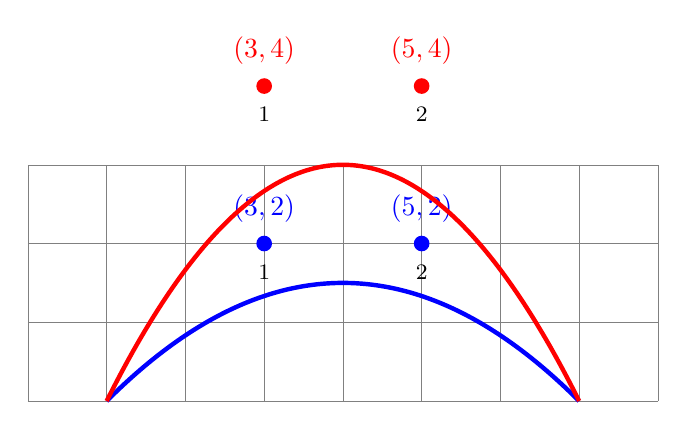
\begin{tikzpicture}[baseline]
\draw[help lines] (0,0) grid (8,3);
\draw[ultra thick,blue] 
  (1,0) 
    .. controls (3,2) and (5,2) .. 
  (7,0) \DrawControl{(3,2)}{blue}{1}\DrawControl{(5,2)}{blue}{2} ;  
\draw[ultra thick,red] 
  (1,0) 
    .. controls (3,4) and (5,4) .. 
  (7,0) \DrawControl{(3,4)}{red}{1}\DrawControl{(5,4)}{red}{2};  
\end{tikzpicture}\hfill
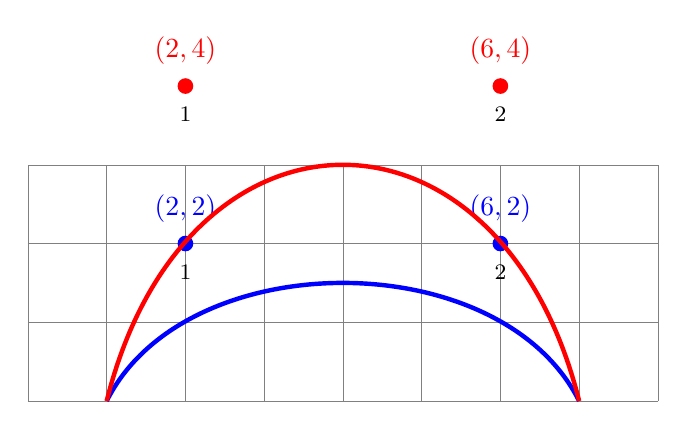
\begin{tikzpicture}[baseline]
\draw[help lines] (0,0) grid (8,3);
\draw[ultra thick,blue] 
  (1,0) 
    .. controls (2,2) and (6,2) .. 
  (7,0) \DrawControl{(2,2)}{blue}{1}\DrawControl{(6,2)}{blue}{2};  
\draw[ultra thick,red] 
  (1,0) 
    .. controls (2,4) and (6,4) .. 
  (7,0) \DrawControl{(2,4)}{red}{1}\DrawControl{(6,4)}{red}{2};  
\end{tikzpicture}

\rule{\textwidth}{2pt}

\vspace{3cm}

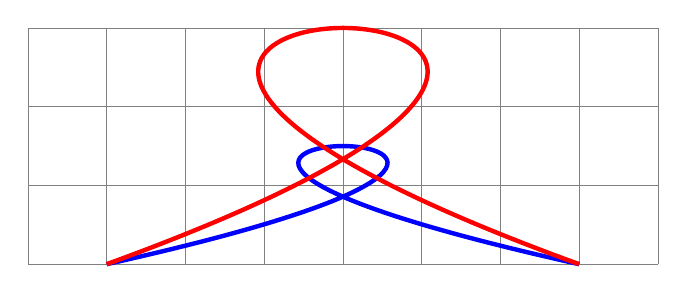
\begin{tikzpicture}[baseline]
\draw[help lines] (0,0) grid (8,3);
\draw[overlay,ultra thick,blue] 
  (1,0) 
    .. controls (10,2) and (-2,2) .. 
  (7,0) \DrawControl{(10,2)}{blue}{1}\DrawControl{(-2,2)}{blue}{2};  
\draw[overlay,ultra thick,red] 
  (1,0) 
    .. controls (12,4) and (-4,4) .. 
  (7,0) \DrawControl{(12,4)}{red}{1}\DrawControl{(-4,4)}{red}{2};  
\end{tikzpicture}

\rule{\textwidth}{2pt}

\begin{tikzpicture}[baseline]
\draw[help lines] (0,-2) grid (8,2);
\draw[ultra thick,blue] 
  (1,0) 
    .. controls (3,2) and (5,-2) .. 
  (7,0) \DrawControl{(3,2)}{blue}{1}\DrawControl{(5,-2)}{blue}{2};  
\draw[ultra thick,red] 
  (1,0) 
    .. controls (-1,5) and (8,-5) .. 
  (7,0) \DrawControl{(-1,5)}{red}{1}\DrawControl{(8,-5)}{red}{2};  
\end{tikzpicture}

\rule{\textwidth}{2pt}

\end{document}